%%%%%%%%%%%%%%%%%%%%%%%%%%%%%%%%%%%%%%%%%%%%%%%%%%%%%%%%%%%%%%%%
%%%%%%%%%%%%%%%%%%%%%%%%%%%%%%%%%%%%%%%%%%%%%%%%%%%%%%%%%%%%%%%%
%%%%
%%%% This text file is part of the source of slides for
%%%% `The Art of HPC, vol 1: The Science of Computing'
%%%% by Victor Eijkhout, copyright 2012-2021
%%%%
%%%%%%%%%%%%%%%%%%%%%%%%%%%%%%%%%%%%%%%%%%%%%%%%%%%%%%%%%%%%%%%%
%%%%%%%%%%%%%%%%%%%%%%%%%%%%%%%%%%%%%%%%%%%%%%%%%%%%%%%%%%%%%%%%

\Level 1 {Derived datatypes}

\begin{frame}[fragile]{Elementary datatypes}
\small\tt\catcode`_=12\relax
  \begin{tabular}{|l|l|l|l|}
    \midrule
    C&&F&\\
    \midrule
    MPI_INT & integer & MPI_INTEGER & Integer \\
    MPI_CHAR & signed char & MPI_CHARACTER & Character \\ 
    MPI_LONG & signed long int&&\\
    MPI_UNSIGNED & unsigned int&&\\
    MPI_FLOAT & float & MPI_REAL & real\\
    MPI_DOUBLE & double & MPI_DOUBLE_PRECISION & Double Precision\\
    MPI_BYTE & & MPI_BYTE & (raw I/O byte)\\
    \midrule
  \end{tabular}
\end{frame}

\begin{frame}[fragile]{Derived datatypes}
  \begin{itemize}
  \item Identify structure in data for efficient transfer
  \item Recursive construction from elementary types
  \item Packing is done for you
  \end{itemize}
\end{frame}

\begin{frame}[fragile]{Derived datatypes}
  \begin{itemize}
  \item Contiguous: contiguous blocks (kinda pointless)
  \item Vector: strided blocks
  \item Indexed: irregular blocks
  \item Struct: Completely general placement and data types
  \end{itemize}
\end{frame}

\begin{frame}[fragile]{Scheme}
\begin{verbatim}
MPI_Type_<type>( oldtype, .... , &newtype );
MPI_Type_commit( newtype );
MPI_Send( .... newtype .... );
MPI_Type_free( newtype );
\end{verbatim}
\end{frame}

\begin{frame}[fragile]{Type signature}
  Signature describes the structure of a datatype

  Send and receive type do not have to be equal:\\
  only be of equal signature

  Example: send 4 doubles, receive one 4-double type
\end{frame}

\begin{frame}{Contiguous}
  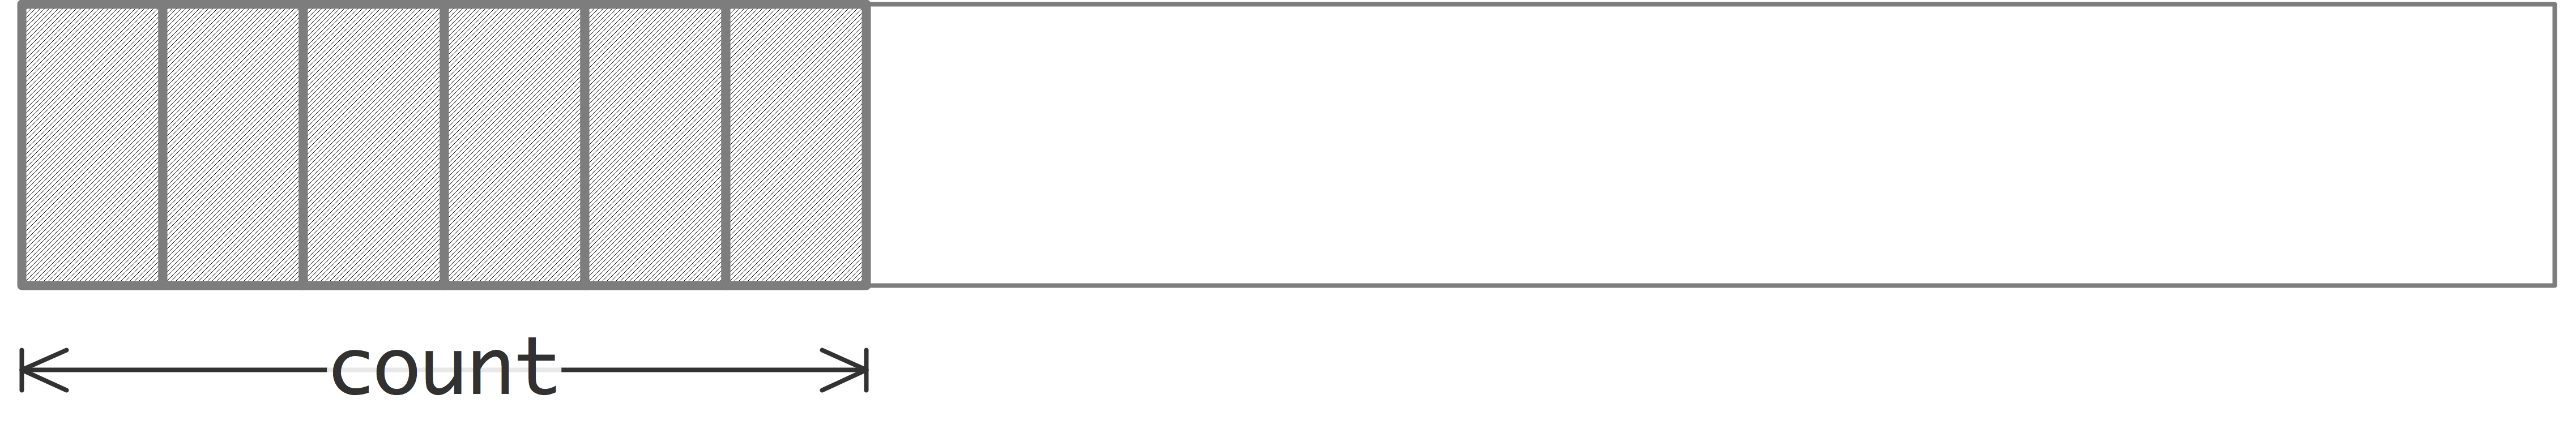
\includegraphics[scale=.06]{data-contiguous}

A contiguous datatype consists of a block of elements of a constituent type
\end{frame}

\begin{frame}[fragile]{Contiguous}
\begin{verbatim}
MPI_Datatype newvectortype;
if (mytid==sender) {
  MPI_Type_contiguous(count,MPI_DOUBLE,&newvectortype);
  MPI_Type_commit(&newvectortype);
  MPI_Send(source,1,newvectortype,receiver,0,comm);
  MPI_Type_free(&newvectortype);
} else if (mytid==receiver) {
  MPI_Status recv_status;
  int recv_count;
  MPI_Recv(target,count,MPI_DOUBLE,sender,0,comm,
    &recv_status);
  MPI_Get_count(&recv_status,MPI_DOUBLE,&recv_count);
  ASSERT(count==recv_count);
}
\end{verbatim}
\end{frame}

\begin{frame}{Vector}
  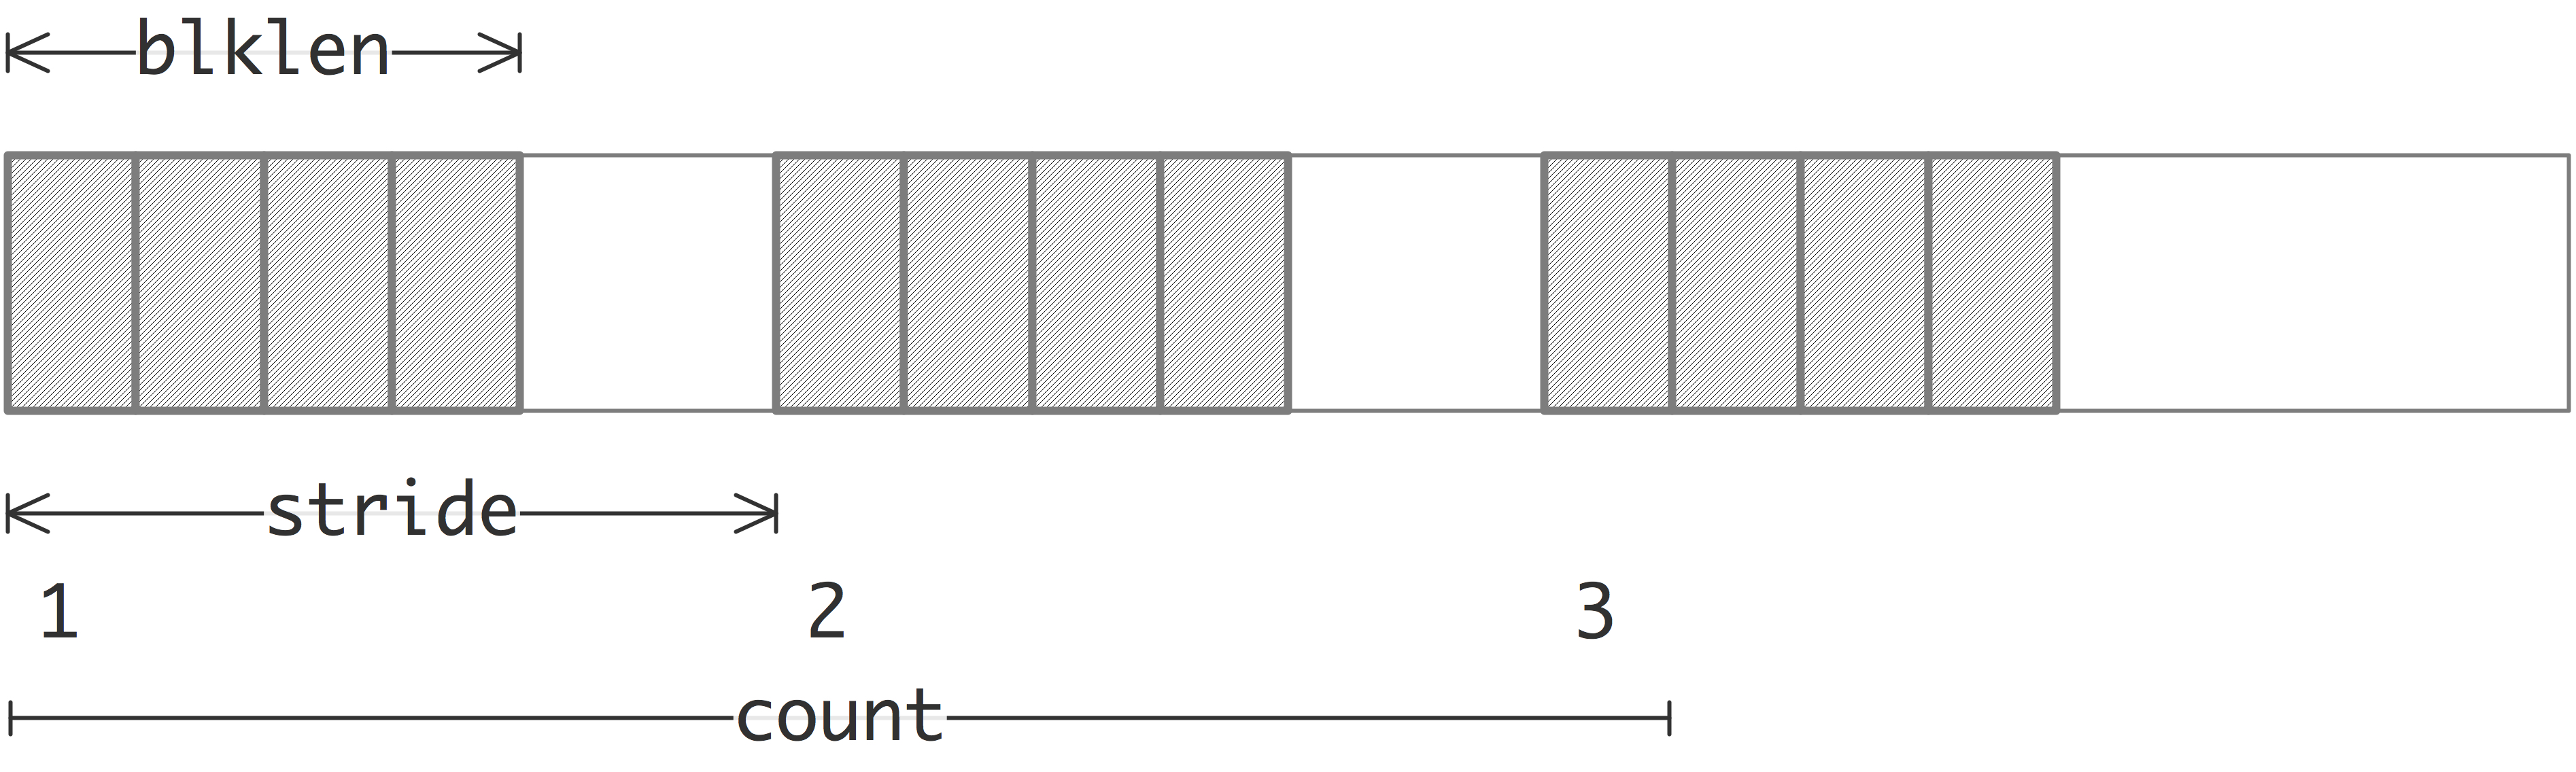
\includegraphics[scale=.09]{data-vector}

A vector datatype is built up out of strided blocks of elements of a constituent type
\end{frame}

\begin{frame}[fragile]{Vector}
\small
\begin{verbatim}
MPI_Datatype newvectortype;
if (mytid==sender) {
  MPI_Type_vector(count,1,stride,MPI_DOUBLE,&newvectortype);
  MPI_Type_commit(&newvectortype);
  MPI_Send(source,1,newvectortype,the_other,0,comm);
  MPI_Type_free(&newvectortype);
} else if (mytid==receiver) {
  MPI_Status recv_status;
  int recv_count;
  MPI_Recv(target,count,MPI_DOUBLE,the_other,0,comm,
    &recv_status);
  MPI_Get_count(&recv_status,MPI_DOUBLE,&recv_count);
  ASSERT(recv_count==count);
}
\end{verbatim}
\end{frame}

\begin{frame}{Indexed / Struct}
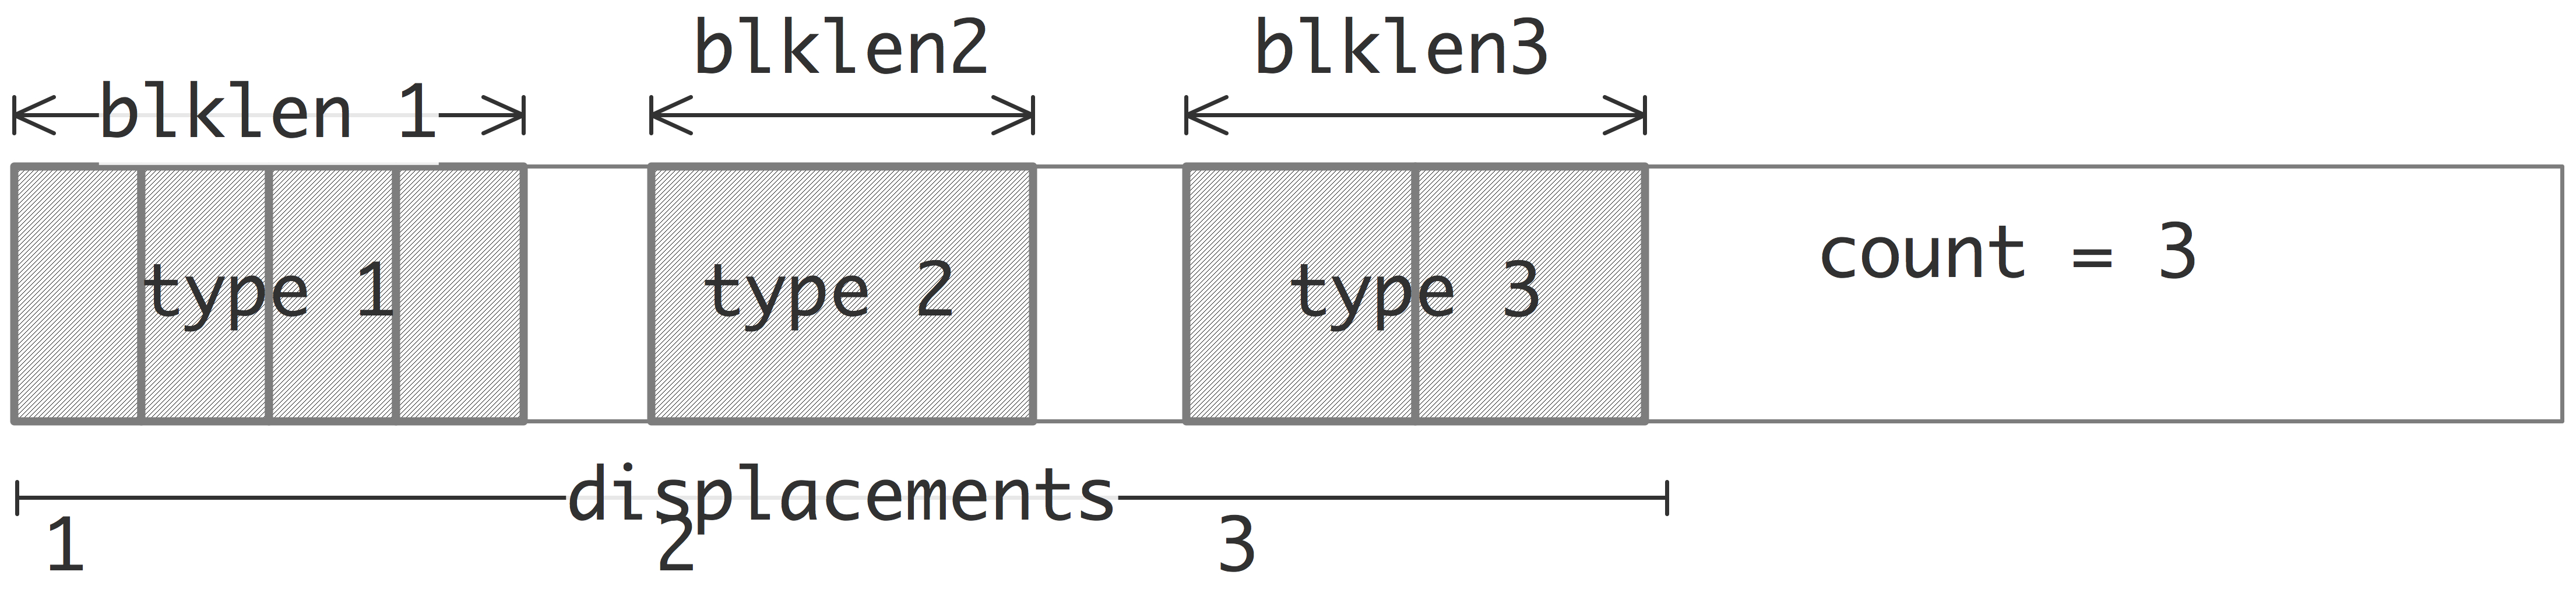
\includegraphics[scale=.07]{data-struct}

Indexed and Struct types have arbitrary blocks with arbitrary
placements; Struct can have multiple types
\end{frame}

\begin{frame}[fragile]{Indexed}
\small %\advance\leftskip by -20pt
\begin{verbatim}
indices = (int*) malloc(count*sizeof(int));
blocklengths = (int*) malloc(count*sizeof(int));
source = (double*) malloc(totalcount*sizeof(double));
target = (double*) malloc(count*sizeof(double));

MPI_Datatype newvectortype;
if (mytid==sender) {
  MPI_Type_indexed(count,blocklengths,indices,MPI_DOUBLE,&newvectortype);
  MPI_Type_commit(&newvectortype);
  MPI_Send(source,1,newvectortype,the_other,0,comm);
  MPI_Type_free(&newvectortype);
} else if (mytid==receiver) {
  MPI_Status recv_status;
  int recv_count;
  MPI_Recv(target,count,MPI_DOUBLE,the_other,0,comm,
    &recv_status);
  MPI_Get_count(&recv_status,MPI_DOUBLE,&recv_count);
  ASSERT(recv_count==count);
}
\end{verbatim}
\end{frame}

\begin{frame}{Struct}
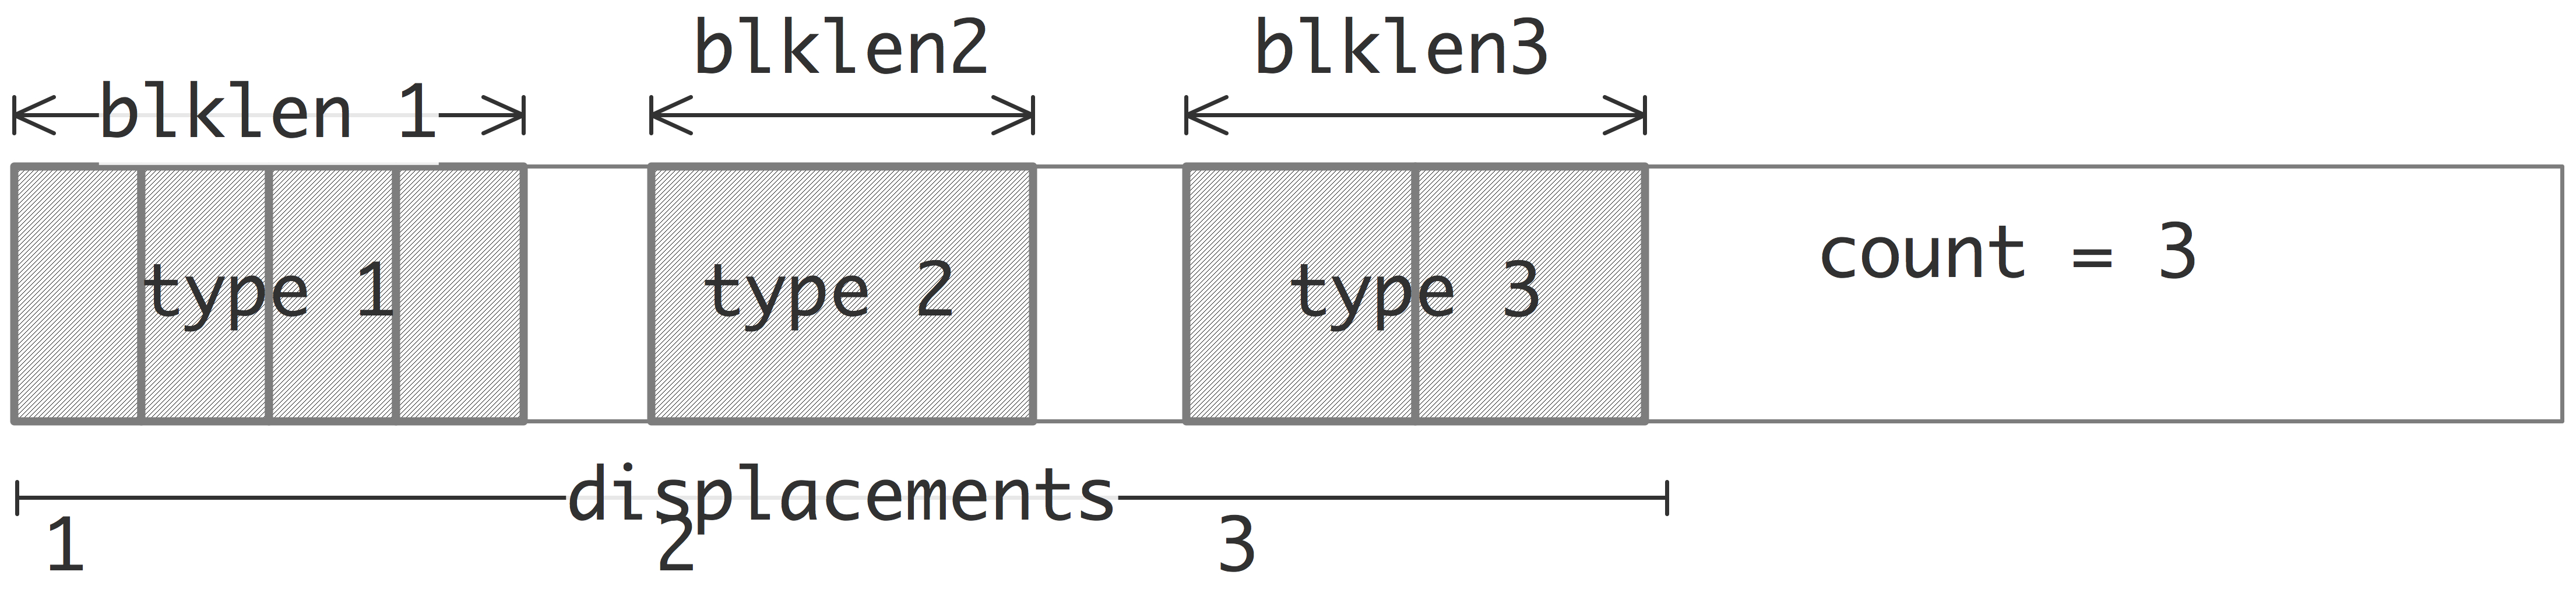
\includegraphics[scale=.07]{data-struct}

Components of a structure are not necessary aligned: \\
tricky location calculations
\end{frame}

\begin{frame}[fragile]{Struct}
\small
\begin{verbatim}
struct object {
  char c;
  double x[2];
  int i;
};

MPI_Datatype newstructuretype;
int structlen = 3;
int blocklengths[structlen]; MPI_Datatype types[structlen];
MPI_Aint displacements[structlen];
// where are the components relative to the structure?
blocklengths[0] = 1; types[0] = MPI_CHAR;
displacements[0] = (size_t)&(myobject.c) - (size_t)&myobject;
blocklengths[1] = 2; types[1] = MPI_DOUBLE;
displacements[1] = (size_t)&(myobject.x[0]) - (size_t)&myobject;
blocklengths[2] = 1; types[2] = MPI_INT;
displacements[2] = (size_t)&(myobject.i) - (size_t)&myobject;
\end{verbatim}
\end{frame}

\begin{frame}[fragile]{Struct (cont'd)}
\small
\begin{verbatim}
MPI_Type_create_struct(
        structlen,blocklengths,displacements,types,
        &newstructuretype);
MPI_Type_commit(&newstructuretype);
{
  MPI_Aint typesize;
  MPI_Type_extent(newstructuretype,&typesize);
  if (mytid==0) printf("Type extent: %d bytes\n",typesize);
}
if (mytid==sender) {
  MPI_Send(&myobject,1,newstructuretype,the_other,0,comm);
} else if (mytid==receiver) {
  MPI_Recv(&myobject,1,newstructuretype,the_other,0,comm,
        MPI_STATUS_IGNORE);
}
MPI_Type_free(&newstructuretype);
\end{verbatim}
\end{frame}

\begin{frame}[fragile]{Packing: another approach to heterogeneous types}
\begin{itemize}
\item The \indexmpishow{MPI_Pack} command adds data to a send buffer;
\item the \indexmpishow{MPI_Unpack} command retrieves data from a receive buffer;
\item the buffer is sent with a datatype of \indexmpishow{MPI_PACKED}.
\end{itemize}
\small
\begin{verbatim}
int MPI_Pack(
  void *inbuf, int incount, MPI_Datatype datatype,
  void *outbuf, int outcount, int *position,
  MPI_Comm comm);
\end{verbatim}
\begin{verbatim}
int MPI_Unpack(
  void *inbuf, int insize, int *position,
  void *outbuf, int outcount, MPI_Datatype datatype,
  MPI_Comm comm);
\end{verbatim}
\end{frame}

\begin{frame}[fragile]{Pack example}
\small
\begin{verbatim}
if (mytid==sender) {
  MPI_Pack(&nsends,1,MPI_INT,buffer,buflen,&position,comm);
  for (i=0; i<nsends; i++) {
    double value = rand()/(double)RAND_MAX;
    MPI_Pack(&value,1,MPI_DOUBLE,buffer,buflen,&position,comm);
  }
  MPI_Pack(&nsends,1,MPI_INT,buffer,buflen,&position,comm);
  MPI_Send(buffer,position,MPI_PACKED,other,0,comm);
\end{verbatim}
\end{frame}

\begin{frame}[fragile]{Pack example (cont'd)}
\small
\begin{verbatim}
} else if (mytid==receiver) {
  int irecv_value;
  double xrecv_value;
  MPI_Recv(buffer,buflen,MPI_PACKED,other,0,comm,
        MPI_STATUS_IGNORE);
  MPI_Unpack(buffer,buflen,&position,&nsends,1,MPI_INT,comm);
  for (i=0; i<nsends; i++) {
    MPI_Unpack(buffer,buflen,&position,&xrecv_value,1,
        MPI_DOUBLE,comm);
  }
  MPI_Unpack(buffer,buflen,&position,&irecv_value,1,
        MPI_INT,comm);
  ASSERT(irecv_value==nsends);
}
\end{verbatim}
\end{frame}

\Level 1 {Communicator manipulation}

\begin{frame}[fragile]{Communicator trickery}
  \begin{itemize}
  \item Communicator duplication
  \item Disjoint subcommunicators
  \item Nondisjoint subcommunicators
  \item Topologies, inter-communicators, spawning (sorry, not in this lecture)
  \end{itemize}
\end{frame}

\begin{frame}[fragile]{Communicator duplication}
  Simplest new communicator: identical copy

  Useful for libraries\\
  separate library traffic from application
\end{frame}

\begin{frame}[fragile]{Comm dup}
\small
\begin{verbatim}
class library {
private:
  MPI_Comm comm;
  int mytid,ntids,other;
  MPI_Request request[2];
public:
  library(MPI_Comm incomm) {
    comm = incomm;
    MPI_Comm_rank(comm,&mytid);
    other = 1-mytid;
  };
  void communication_start() {
    int sdata=6,rdata;
    MPI_Isend(&sdata,1,MPI_INT,other,2,comm,&(request[0]));
    MPI_Irecv(&rdata,1,MPI_INT,other,MPI_ANY_TAG,comm,&(request[1])); }
  void communication_end() {
    MPI_Status status[2];
    MPI_Waitall(2,request,status); }
};
\end{verbatim}
\end{frame}

\begin{frame}[fragile]{Comm dup (cont'd)}
\small
\begin{verbatim}
MPI_Isend(&sdata,1,MPI_INT,other,1,comm,&(request[0]));
my_library.communication_start();
MPI_Irecv(&rdata,1,MPI_INT,other,MPI_ANY_TAG,comm,
          &(request[1]));
MPI_Waitall(2,request,status);
my_library.communication_end();
\end{verbatim}
\end{frame}

\begin{frame}[fragile]{Communicator splitting}
Processor grid:
\begin{verbatim}
MPI_Comm_rank( &mytid );
proc_i = mytid % proc_column_length;
proc_j = mytid / proc_column_length;
\end{verbatim}
Communicator per column:
\begin{verbatim}
MPI_Comm column_comm;
MPI_Comm_split( MPI_COMM_WORLD, proc_j, i, &column_comm );
\end{verbatim}
Broadcast in that column:
\begin{verbatim}
MPI_Bcast( data, /* tag: */ 0, column_comm );
\end{verbatim}
\end{frame}

\begin{frame}[fragile]{Comm split example}
\small
\begin{verbatim}
MPI_Comm_size(comm,&npes);
MPI_Comm_rank(comm,&rank);
int icolor = rank%3, key = npes-rank;

MPI_Comm_split(comm,icolor,key,&newcomm);
MPI_Comm_rank(newcomm,&newrank);
\end{verbatim}

\begin{tabular}{|lllll|}
\midrule
rank&icolor&key&newrank&color zero\\ \midrule
0&0&9&2&$\Leftarrow$\\
1&1&8&2&\\
2&2&7&2&\\
3&0&6&1&$\Leftarrow$\\
4&1&5&1&\\
5&2&4&1&\\
6&0&3&0&$\Leftarrow$\\
7&1&2&0&\\
8&2&1&0&\\
\midrule
\end{tabular}
\end{frame}

\begin{frame}[fragile]{Communicators and groups}
Communicator to group to communicator:
\begin{verbatim}
MPI_Comm_group( comm, &group);
MPI_Comm_create( old_comm, group, &new_comm );
\end{verbatim}
and groups are manipulated with
\indexmpishow{MPI_Group_incl}, \indexmpishow{MPI_Group_excl},
\indexmpishow{MPI_Group_difference} and a few more.
\end{frame}

\Level 1 {Non-blocking collectives}
 
\begin{frame}{General idea}
\begin{itemize}
\item Collectives are blocking
\item Any process delay visible to every other process
\item Some architectures have separate network for collectives
\item Idea: let collective progress independently, test for completion
\end{itemize}
\end{frame}

\begin{frame}[fragile]{Example}
Non-blocking collective gives \verb+MPI_Request+ pointer
\begin{verbatim}
int MPI_Iallreduce(const void *sendbuf, void *recvbuf, 
    int count, MPI_Datatype datatype, 
    MPI_Op op, MPI_Comm comm, 
    MPI_Request *request)
\end{verbatim}
Test for completion with \verb+MPI_Wait+ and \verb+MPI_Test+ and such.
\end{frame}

\begin{frame}{Latency hiding}
Overlapping collective communication with useful computation,

Example: in iterative methods
\[ 
\begin{array}{l}
x\leftarrow\cdots\\
x^tx\quad\hbox{non-blocking start}\\
y\leftarrow Ax\\
y\leftarrow y/x^tx
\end{array}
\]
\end{frame}

\Level 1 {One-sided communication}

\begin{frame}[fragile]{Basic notions}
\begin{itemize}
\item One-sided access: Put, Get, Accumulate
\item Window: memory designated for one-sided communication
\item Origin: process that makes the one-sided call\\
  target: process that exposes memory window
\item Different synchronization mechanism: active and passive target synchronization
\item Memory model: shared memory explicitly synchronized with local memory
\end{itemize}
\end{frame}

\begin{frame}[fragile]{Windows}
\small
\begin{verbatim}
MPI_Win_create (void *base, MPI_Aint size, 
  int disp_unit, MPI_Info info, 
  MPI_Comm comm, MPI_Win *win)
\end{verbatim}
  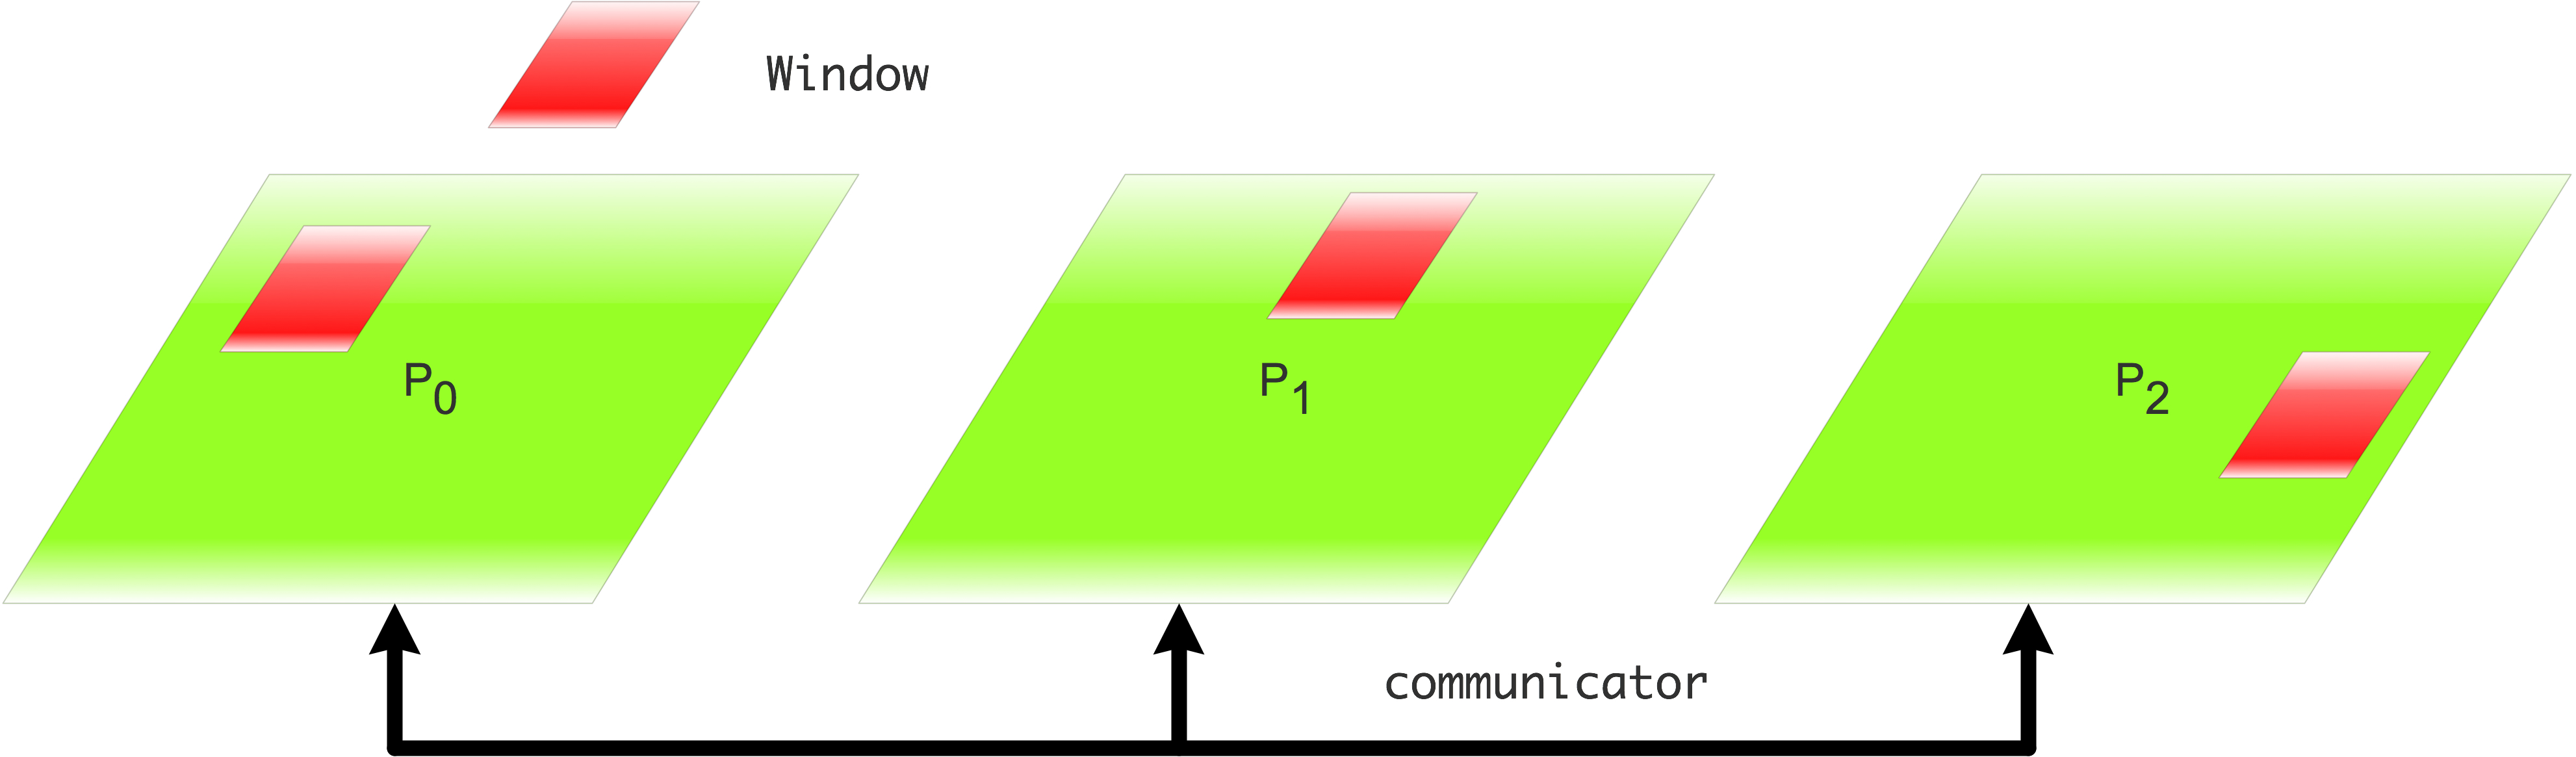
\includegraphics[scale=.08]{one-sided-window}

Note: collective on communicator
\end{frame}

\begin{frame}[fragile]{Put/Get/Accumulate}
\small
\begin{verbatim}
MPI_Put (void *origin_addr, int origin_count, 
  MPI_Datatype origin_datatype, int target_rank,
  MPI_Aint target_disp, int target_count, 
  MPI_Datatype target_datatype,
  MPI_Win window)
\end{verbatim}
\begin{verbatim}
MPI_Accumulate (void *origin_addr, int origin_count, 
  MPI_Datatype origin_datatype, int target_rank,
  MPI_Aint target_disp, int target_count, 
  MPI_Datatype target_datatype,
  MPI_Op op,MPI_Win window)
\end{verbatim}
\end{frame}

\begin{frame}[fragile]{Globally defined epochs}
\begin{verbatim}
MPI_Win_fence((MPI_MODE_NOPUT | MPI_MODE_NOPRECEDE), win);
MPI_Get( /* operands */, win);
MPI_Win_fence(MPI_MODE_NOSUCCEED, win);
\end{verbatim}
Induces synchronization
\end{frame}

\begin{frame}{Restrictions from memory model}
Windows are not coherent with local memory:
\begin{itemize}
\item Data in window undefined until fence synchronization
\item No put and get in same epoch
\end{itemize}
\end{frame}

\begin{frame}[fragile]{Fine-grained synchronization}
\small
Exposure:
\begin{verbatim}
MPI_Win_post( /* group of origin processes */ )
MPI_Win_wait()
\end{verbatim}
Access:
\begin{verbatim}
MPI_Win_start( /* group of target processes */ )
// access operations
MPI_Win_complete()
\end{verbatim}
\end{frame}

\begin{frame}[fragile]{Example}
\small
\begin{verbatim}
if (mytid==origin) {
  MPI_Group_incl(all_group,1,&target,&two_group);
  // access
  MPI_Win_start(two_group,0,the_window);
  MPI_Put( /* data on origin: */   &my_number, 1,MPI_INT,
   /* data on target: */   target,0,   1,MPI_INT,
	   the_window);
  MPI_Win_complete(the_window);
}
if (mytid==target) {
  MPI_Group_incl(all_group,1,&origin,&two_group);
  // exposure
  MPI_Win_post(two_group,0,the_window);
  MPI_Win_wait(the_window);
}
\end{verbatim}
\end{frame}

\begin{frame}[fragile]{Passive target synchronization}
\begin{verbatim}
If (rank == 0) {
  MPI_Win_lock (MPI_LOCK_EXCLUSIVE, 1, 0, win);
  MPI_Put (outbuf, n, MPI_INT, 1, 0, n, MPI_INT, win);
  MPI_Win_unlock (1, win);
}
\end{verbatim}
Lock types are:
\begin{itemize}
\item \texttt{MPI_LOCK_SHARED} for Get;
\item \texttt{MPI_LOCK_EXCLUSIVE} for Put and Accumulate
\end{itemize}
\end{frame}

\begin{frame}[fragile]{Start/complete/post/wait example}
\small
\begin{verbatim}
if (mytid==origin) {
  MPI_Group_incl(all_group,1,&target,&two_group);
  // access
  MPI_Win_start(two_group,0,the_window);
  MPI_Put( /* data on origin: */   &my_number, 1,MPI_INT,
   /* data on target: */   target,0,   1,MPI_INT,
	   the_window);
  MPI_Win_complete(the_window);
}

if (mytid==target) {
  MPI_Group_incl(all_group,1,&origin,&two_group);
  // exposure
  MPI_Win_post(two_group,0,the_window);
  MPI_Win_wait(the_window);
}
\end{verbatim}
\end{frame}

\begin{frame}{Passive target synchronization}
\begin{itemize}
\item Emulates shared memory
\item Origin process locks window on target
\item MPI-2 was lacking atomic operations
\item MPI-3 has the fix
\end{itemize}
\end{frame}

\begin{frame}[fragile]{Passive target example}
\small
\begin{verbatim}
for (int i=0; i<ninputs; i++) 
  myjobs[i] = 0;
if (mytid!=repository) {
  float contribution=(float)mytid,table_element;
  int loc=0;
    MPI_Win_lock(MPI_LOCK_EXCLUSIVE,repository,0,the_window);
    // read the table element by getting the result from adding zero
    err = MPI_Fetch_and_op(&contribution,&table_element,MPI_FLOAT,
     	            repository,loc,MPI_SUM,the_window); CHK(err);
    MPI_Win_unlock(repository,the_window);
}
\end{verbatim}
\end{frame}

\begin{frame}[fragile]{MPI\_T tool interface}
VarList: list internal variables
\texttt{https://computation-rnd.llnl.gov/mpi_t/varList.php}

Gyan: monitor internal variables
\texttt{https://computation-rnd.llnl.gov/mpi_t/gyan.php}
\end{frame}
